\documentclass{beamer}
%Information to be included in the title page:
\title{Reverse Mode Algorithmic Differentiation}
\author[Group 18]{Callum Firth, Maximilian Fricker, Alexander Le Marchant, Samuel Murdoch}
\institute[Imperial]{Imperial College London}
\date{20th June 2023}
\usetheme{Madrid}

\begin{document}

\frame{\titlepage}

% This may all change but:


% Intro
% Im thinking we start with a brief overview on why care about derivatives and the types of func we are caring about (ie. these are the R^n to R^1 func or similar)
% Then maybe move to the DAG representation of expressions (Talk about how we did this, why dag better)
% 

% RM
% See if we can create a gif? of a traversal of a DAG
% Show both the forward pass to evaluate it and then the backward pass
% Then maybe compare this to the forward mode gif
% Breifly mention complexity of the two algorithms (maybe only care about time here)
% Then talk about difference in time of the two algorithms

% Demo (May swap with conclusion/applications)
% Show basic derivative calculation (think of a nice function so we can easily confirm this)
% Move on to show difference in time between RM and FM (can be for a simple ex of n = 50)
% If completed in time show ODE equation/simulation

% Conclusion/Applications
% Mention theory behind ODE stuff
% Mention theory why we care about the neural network stuff
% Talk about neural networks maybe application on backpropagation, reducing loss func, optimising weights etc

\AtBeginSection[Introduction]
{
\begin{frame}{Outline}
    \tableofcontents[currentsection]
\end{frame}
}

\section{Introduction}

\begin{frame}{Why are Derivatives important?}
\frametitle{Why are Derivatives Important?}
Motivation, neural networks, gradient descent
\end{frame}

\begin{frame}{Types of Differentiation}
\frametitle{Types of differentiation}
Three common ways to differentiate a function on a computer
\begin{itemize}
    \item Finite Differences
    \item Symbolic Differentiation
    \item Algorithmic Differentiation (AD)
\end{itemize}
\end{frame}

\begin{frame}{Function Definition}
    \begin{equation*}
            F: \mathbb{R}^n \longrightarrow \mathbb{R}^m \qquad
            F(x_1, \ldots, x_n) = (y_1, \ldots, y_m)
    \end{equation*}
    We will compare the computational costs of the Jacobian of $F$
    \begin{equation*} \label{jacobian}
        F'(x) = \begin{bmatrix}
            \frac{\partial y_1}{\partial x_1} & \cdots & \frac{\partial y_1}{\partial x_n} \\
            \vdots & \ddots & \vdots \\
            \frac{\partial y_m}{\partial x_1} & \cdots & \frac{\partial y_m}{\partial x_n}
        \end{bmatrix} \in \mathbb{R}^{m \times n}
    \end{equation*}
    Cost to compute $F$ is $\mathcal{O}(\mu)$
\end{frame}


\begin{frame}{Finite Differences}
    \begin{equation*}
        \frac{\partial F_i (p)}{\partial x_j} \approx \frac{F_i(p+he_j) - F_i(p)}{h}
    \end{equation*}
    \begin{itemize}
        \item Uses a truncated Taylor expansion 
        \item Returns \alert{approximate} value
        \item Low computational costs
        \begin{itemize}
            \item $\mathcal{O}(n \mu)$
        \end{itemize}
    \end{itemize}
\end{frame}

\begin{frame}{Symbolic Differentiation}
    \begin{itemize}
        \item Uses computer algebra packages to take derivatives
        \begin{itemize}
            \item Application of chain rule
        \end{itemize}
        \item Calculates derivative at all $x \in \mathbb{R}^n$
        \item Once solution found any value can be plugged in
        \item Returns \alert{exact} value
        \item Very high computational cost
        \begin{itemize}
            \item $\mathcal{O}(nm \mu)$
        \end{itemize}
    \end{itemize}
\end{frame}

\begin{frame}{Algorithmic Differentiation}
    \begin{itemize}
        \item Two types
            \begin{itemize}
                \item Forward mode
                \item Reverse mode - we will focus on reverse mode
            \end{itemize}
        \item Application of chain rule
        \item Calculates derivative at specified $x \in \mathbb{R}^n$
        \item Returns \alert{exact} value up to machine precision
        \item Low computational costs
            \begin{itemize}
                \item $\mathcal{O}(n \mu)$ with forward mode
                \item $\mathcal{O}(m \mu)$ with reverse mode
            \end{itemize}
    \end{itemize}
\end{frame}

\AtBeginSection[Reverse Mode Algorithmic Differentiation]
{
\begin{frame}{Outline}
    \tableofcontents[currentsection]
\end{frame}
}

\section{Reverse Mode Algorithmic Differentiation}

\begin{frame}{Expressions as Trees}
\frametitle{Expressions as Trees}
Simple maybe 3 inputs 1 output
\end{frame}

\begin{frame}{Expressions as Directed Acylic Graphs}
    \frametitle{Expressions as Directed Acylic Graphs}
\end{frame}

\begin{frame}{Reverse Mode AD}
    \begin{equation*} \label{1df}
            f: \mathbb{R} \longrightarrow \mathbb{R} \qquad
            f(x) = (y)
    \end{equation*}
    \begin{figure}
        \centering
        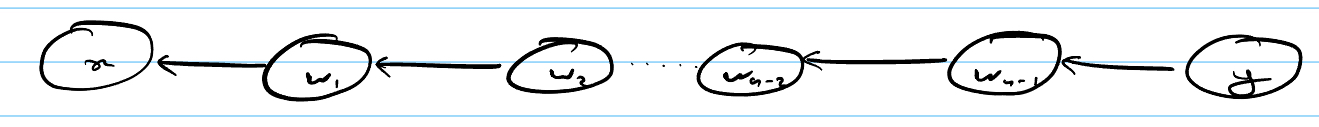
\includegraphics[width=10cm]{images/1d_func_sketch.jpg}
    \end{figure}
    Applying chain rule
    \begin{equation*}
        \begin{split}
            \frac{\partial y}{\partial x} & = \frac{\partial y}{\partial w_{1}} \frac{\partial w_{1}}{\partial x} \\
            \onslide<2->{& = \frac{\partial y}{\partial w_{2}} \frac{\partial w_{2}}{\partial w_{1}} \frac{\partial w_{1}}{\partial x}} \\
            \onslide<3->{& = \ldots \\
            & = \frac{\partial y}{\partial w_{n-1}} \frac{\partial w_{n-1}}{\partial w_{n-2}} \cdots \frac{\partial w_2}{\partial w_1} \frac{\partial w_1}{\partial x}}
        \end{split}
    \end{equation*}
\end{frame}

\begin{frame}{Reverse Mode AD}
    Quantity of importance is the \alert{adjoint} $\Bar{w}_i$
    \begin{equation*}
        \Bar{w}_i = \frac{\partial y}{\partial w_i}
    \end{equation*}
    Calculation from previous slide can be rewritten as
    \begin{equation*}
        \begin{split}
            \frac{\partial y}{\partial x} & = \Bar{w}_1 \frac{\partial w_{1}}{\partial x} \\
            \onslide<2->{& = \Bar{w}_2 \left( \frac{\partial w_{2}}{\partial w_{1}} \frac{\partial w_{1}}{\partial x} \right) } \\
            \onslide<3->{& = \ldots \\
            & = \Bar{w}_{n-1} \left( \frac{\partial w_{n-1}}{\partial w_{n-2}} \cdots \frac{\partial w_2}{\partial w_1} \frac{\partial w_1}{\partial x} \right)}
        \end{split}
    \end{equation*}
    \onslide<4->{As we traverse the graph we store the adjoints}
\end{frame}

\begin{frame}{Adjoints of Standard Functions}
    \begin{table}[h!]
    \centering
    \begin{tabular}{|lll|}
        \hline
        Function & $\Bar{x}$ & $\Bar{y}$ \\
        \hline
        $x+y$ & $1$ & $1$ \\
        $x-y$ & $1$ & $-1$ \\
        $x \times y$ & $y$ & $x$ \\
        $x / y$ & $1/y$ & $-x/y^2$ \\
        $x^y$ & $y{x}^{(y-1)}$ & ${x}^{y}\log(x)$ \\
        $\sin(x)$ & $\cos(x)$ &  \\
        $\cos(x)$ & $-\sin(x)$ &  \\
        $\exp(x)$ & $\exp(x)$ &  \\
        $\log(x)$ & $1/x$ &  \\
        \hline
    \end{tabular}
    \label{tab:Adjelementals}
    \end{table}
\end{frame}

\begin{frame}{Forward Pass}
\frametitle{Forward Pass}
DAG gif forward pass
\end{frame}

\begin{frame}{Reverse Pass}
\frametitle{Reverse Pass}
DAG gif reverse pass
\end{frame}

\begin{frame}{Time Complexity}
\frametitle{??Time complexity?? demo??}
Difference in FM and RM?
\end{frame}

\begin{frame}{Demo}
\frametitle{Demo 1}
Demo that what we have works
\end{frame}

\begin{frame}{Numpy Demo}
\frametitle{What if we want more than 1 output}
Show new DAG
Numpy arr implemenentation talk
\end{frame}

\begin{frame}
\frametitle{??Time complexity?? Demo??}
Time difference in FM and RM
\end{frame}

\begin{frame}{Further Applications}
\frametitle{Further Applications}
If we want to solve adjoint of PDE
\end{frame}

\begin{frame}
\frametitle{Advection Diffusion Equation}
Talk about initial setup
\end{frame}

\begin{frame}
\frametitle{More: Advection diffusion equation}
Maybe show gif or picture of the graph over time
This show implementations
How do we know we are correct
\end{frame}

\begin{frame}
\frametitle{Adjoint of this}
Now the adjoint of this
\end{frame}

\begin{frame}
\frametitle{Demo}
How does this work with our code/work
\end{frame}

\begin{frame}
\frametitle{??Conclusion??}
How does this work with our code/work
\end{frame}

\end{document}